\providecommand{\main}{..}
\documentclass[\main/main.tex]{subfiles}

\begin{document}
    \justify
    W celu zweryfikowania wyników otrzymanych w poprzednich badaniach, przeprowadzono trening perceptronu prostego oraz Adaline przy takich samych wartościach hiperparametrów. Wybrany współczynnik uczenia się wynosi 0.1, parametr theta ma natomiast wartość 0.5. Wagi początkowe wygenerane zostały natomiast z przedziału [-0.2, 0.2]. W przypadku perceptronu prostego uruchomiono pomiary zarówno dla funkcji unipolarnej jak i bipolarnej.
    
    \begin{figure}[H]
    \centering
    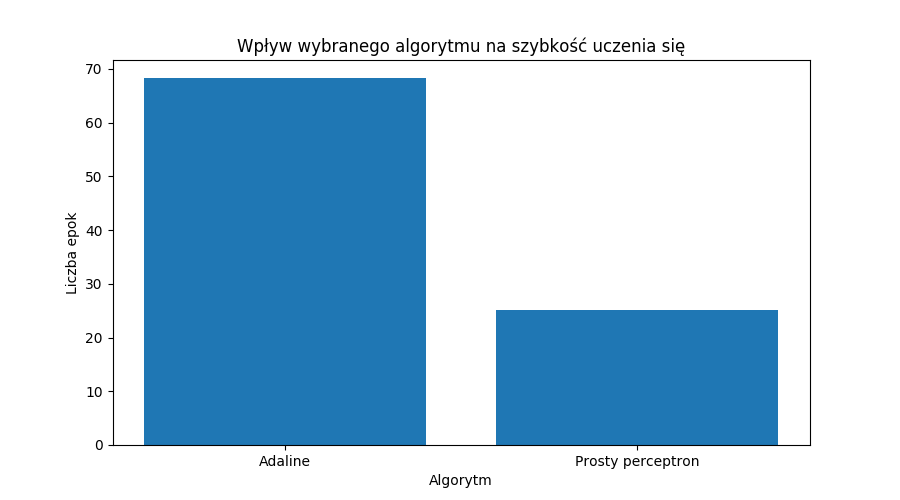
\includegraphics[scale=0.6]{test_algorithms_100}
    \caption{Porównanie wymaganej liczby epok dla różnych algorytmów}
    \end{figure}
    
    \paragraph{}
    Na powyższym wykresie widocznym jest, że obie wersje perceptronu prostego, zarówno ta wykorzystująca unipolarną funkcję aktywacji jak i bipolarną, osiągają znacznie lepsze wyniki średnie niż Adaline. Związane jest to z obserwacjami pojawiającymi się w poprzednich badaniach. W przypadku Adaline wartości wag początkowych nie są tak samo ważne jak w przypadku perceptronu prostego, ponieważ Adaline i tak zawsze zmierza do ustanowienia tych samych wag. Jednocześnie to, że w trakcie uczenia, nie transformujemy wyników predykcji przy użyciu funkcji aktywacji powoduje, że zmiany w wagach mogą być bardzo gwałtowne przez co algorytm wymaga więcej czasu na odpowiednie dopasowanie.
    Tak jak zauważono w poprzednich badaniach, w przypadku perceptronu prostego, bipolarna funkcja aktywacji osiąga lepsze wyniki niż unipolarna. Nie jest to jednak tak gwałtowna różnica jak w przypadku Adaline.
    
\end{document}
